\documentclass[skript.tex]{subfiles}

\begin{document}
	\setcounter{cntr}{62}
	\begin{bsp}
		Sei $X=\mbb{R}^2,\ \Sigma = \mc{B}^2,\ f(x,y)=\frac{x-y}{(x+y)^3}$. Wir betrachten das Riemann-Integral
		\[
			\int_0^1 \int_0^1 f(x,y) \md x \md y \stackrel{\footnotemark}{=} - \int_0^1 \frac{\md y}{(1+y)^2} = \frac{1}{1+y} \bigg\vert_0^1 = -\frac{1}{2}
		\] \footnotetext{$\frac{\md}{\md x} \frac{x}{(x+y)^2} = \frac{1}{(x+y)^2}-2\frac{x}{(x+y)^3} = \frac{x-y}{(x+y)^3}\ \mathrm{ und }\ \int_0^1 \int_0^1 f(x,y) \md x \md y = \frac{1}{2}$}
		Wäre $f\in \mathscr{L}^1\pr{[0,1]^2}$, so folge aus dem \textup{Satz 62 (Fatou)} zunächst die Integrierbarkeit der Funktionen
		\[
			\int_{(0,1)} f(x_1,\cdot) \md \lambda(x_1),\ \int_{(0,1)} f(\cdot, x_2) \md \lambda(x_2) 
		\]
		und da $f$ auf $(0,1)\times(0,1)$ stetig ist, erhalten wir Übereinstimmung von Lebesgue- und Riemann-Integral und erneut mit \textup{Satz 62}
		\[
			\iint f(x_1, x_2) \md x_1 \md x_2 = \iint f(x_1, x_2) \md x_2 \md x_1. \quad \lightning % maybe something is wrong here.....
		\]
	\end{bsp}
	
	\begin{lem}
		Seien $(X_1, \Sigma_1),(X_2, \Sigma_2)$ Messräume und $S_1 \sbs \Sigma_1,\ S_2 \sbs \Sigma_2$ mit\\ $\Sigma_{X_1}(S_1) = \Sigma_1,\ \Sigma_{X_2}(S_2) = \Sigma_2$. Dann gilt
		\[
			\underbrace{\Sigma_1 \otimes \Sigma_2}_{\substack{\sigma\text{-Algebra erzeugt von }\\ A_1\times A_2,\ A_j \in \Sigma_j}} \stackrel{\substack{\supset \text{ haben} \\ \text{wir schon} \\ \downarrow}}{=} \underbrace{\Sigma_{X_1 \times X_2}\pr{S_1 \times S_2}}_{\substack{\sigma\text{-Algebra erzeugt von }\\ A_1\times A_2,\ A_j \in S_j}}\quad \Sigma , \mathrm{\rotatebox[origin=c]{180}{$\ceq$}}
		\]
		wobei $S_1 \times S_2 = \cbr{A_1 \times A_2 \mid A_1 \in S_1,\ A_2 \in S_2}$.
	\end{lem}
	
	\begin{proof}
		\hfill
		\begin{itemize}
			\item[''$\supset$''] klar.
			\item[''$\subset$''] Die Menge $\cbr{A_1 \in \Sigma_1 \mid A_1 \times X_1 \in \Sigma}$ ist eine $\sigma$-Algebra (nachrechnen!), die $S_1$ enthält, also identisch mit $\Sigma_1$. Insbesondere mit $\Sigma_1 \times X_2 \stackrel{\text{def}}{=} \cbr{A_1 \times X_2 \mid A_1 \in \Sigma_1} \sbs \Sigma$, ebenso gilt $X_1 \times \Sigma_2 \sbs \Sigma$. Nun folgt
			\begin{align*}
				\Sigma_1 \times \Sigma_2 &= \cbr{A_1 \times A_2 \mid A_1 \in \Sigma_1,\ A_2 \in \Sigma_2}\\
				&= \cbr{(A_1\times X_2) \cap (X_1 \times A_2) \mid A_1 \in \Sigma_1,\ A_2 \in \Sigma_2} \\
				&\stackrel{\text{def}}{=} \pr{\Sigma_1 \times X_2} \cap \pr{X_1 \times \Sigma_2} \sbs \Sigma
			\end{align*} 
			Weil $\Sigma$ eine $\sigma$-Algebra ist, folgt $\Sigma_1 \otimes \Sigma_2 \sbs \Sigma$.
		\end{itemize}
	\end{proof}
	
	\begin{lem}
		Gegeben seien Maßräume $\pr{X_j, \Sigma_j, \mu_j},\ j=1,2,3$, mit $\sigma$-finiten Maßen. Dann gilt $\pr{\Sigma_1 \otimes \Sigma_2} \otimes \Sigma_3 = \Sigma_1 \otimes \pr{\Sigma_2 \otimes \Sigma_3}$ und $\pr{\mu_1 \otimes \mu_2} \otimes \mu_3 = \mu_1 \otimes \pr{\mu_2 \otimes \mu_3}$.
	\end{lem}

	\begin{proof}
		Die erste Identität folgt, weil beide Seiten jeweils von Mengen $A_1 \times A_2 \times A_3,\ A_j \in \Sigma_j$ erzeugt werden. Darüber hinaus stimmen die beiden Maße wegen
		\begin{align*}
		\pr{\pr{\mu_1 \otimes \mu_2} \otimes \mu_3}\pr{A_1 \times A_2 \times A_3} &= \mu_1(A_1) \mu_2(A_2) \mu_3(A_3)\\
		&= \pr{\mu_1 \otimes \pr{\mu_2 \otimes \mu_3}}\pr{A_1 \times A_2 \times A_3}
		\end{align*}
		auf allen ''Rechtecken'' überein und damit nach \textit{Satz 23 (Eindeutigkeit)} überall.
	\end{proof}
	
	\begin{theorem}[Lebesgue-Maß]
		Das durch $\lambda^n \ceq \lambda_1 \otimes \lambda_2 \otimes \dotsc \otimes \lambda_n$ definierte Lebesgue-Maß auf $\mbb{R}^n$ besitzt die folgenden Eigenschaften (im Folgenden verwenden wir immer die Borel-$\sigma$-Algebra)
		\begin{itemize}
			\item[(i)] Durch die Werte auf der Menge $\mc{I}$ sämtlicher Quader der Form $I=\mathop{\bigtimes}_{j=1}^{n} I_j$, wobei $I_j$ Intervalle sind, ist $\lambda^n$ eindeutig bestimmt. 
			
			\item[(ii)] Für jedes $B \in \mc{B}^n$ gilt:
				\[
				\lambda^n(B) = \inf \cbr{\sum_{k\in\N} \lambda^n(A_k) \: \bigg| \: (A_k)_{k\in\N} \sbs \mc{I},\ B \sbs \bigcup_{k\in\N} A_k}
				\]
			(vgl. \textup{Lemma 30}).
			
			\item[(iii)] Das Maß $\lambda^n$ ist translationsinvariant und bis auf Normierung das einzige Borelmaß mit dieser Eigenschaft.
		\end{itemize}
	\end{theorem}
	
	\begin{bem*}
		Das Produktmaß zweier vollständiger Maße (\textup{Bem. 29}) ist i.A. nicht vollständig. 
	\end{bem*}

	\begin{proof}[Beweis Lebesgue-Maß]
		\hfill
		\begin{itemize}
			\item[(i)] Da $\mc{I}$ unter Schnitten abgeschlossen ist, und wegen \textit{Lemma 64} die Borel-$\sigma$-Algebra $\mc{B}^n$ erzeugt, folgt die Behauptung mit dem Eindeutigkeitssatz (23).
			
			\item[(ii)] Sei $\mc{A}$ die Algebra (nachrechnen!) endlicher Vereinigungen disjunkter Quader aus $\mc{I}$. Nun ist $\mu \ceq \lambda^n \vert_\mc{A}$ ein Prämaß. Die angegebene Formel ist gerade die Konstruktion des äußeren Maßes in \textit{Lemma 30}, und mit \textit{Satz 28} erhalten wir eine $\sigma$-Algebra $\Sigma$ mit $\mc{A} \in \Sigma$, sodass $\pr{\mbb{R}^n, \Sigma, \mu^*\vert_\Sigma}$ ein Maßraum ist. Weil $\mc{A}$ sämtliche offenen Quader $\bigtimes_{j=1}^n (a_j,b_j)$ enthält, folgt $\mc{B}^n = \Sigma_{\mbb{R}^n} (\mc{A}) \sbs \Sigma$ und $\mu^*\vert_{\mc{B}^n}$ ist ein Maß auf $\mc{B}^n$, was zu zeigen war.
			
			\item[(iii)] Die Translationsinvarianz ergibt sich unmittelbar aus (ii). Sei nun $\mu$ ein weiteres translationsinvariantes Maß auf $(\mbb{R}^n, \mc{B}^n)$. Sei $Q_r$ ein halboffener Würfel mit Seitenlänge $r$. Wir nehmen \OE\ $\mu(Q_1)=1$ an. Weil wir $Q_1$ in $m^n$ Würfel der Kantenlänge $\frac{1}{m}$ zerlegen können, folgt mit Translationsinvarianz und Additivität des Maßes:
			\[
				1 = \mu(Q_1) = m^n \mu\pr{Q_{\frac{1}{m}}} = m^{-n}. 
				\qquad \qquad
				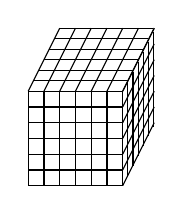
\begin{tikzpicture}
					\foreach \x in {0,1,...,6}{
						\draw (\x / 5, 0) -- (\x / 5, 6/5);
						\draw (\x / 5, 6/5) -- (\x/5 + 0.4, 10/5 ); 
					};
					
					\foreach \y in {0,1,...,6}{
						\draw (0, \y/5) -- (6/5, \y/5);
						\draw (6/5, \y/5) -- (8/5, \y/5 + 0.8);
					};
					\foreach \x in {1,2,...,6} {
						\draw (\x/5 -0.135*\x, \x / 7.5 + 6/5) -- (\x / 5 + 6/5 - 0.135*\x, \x / 7.5 + 6/5);
					};
					\foreach \x in {0,1,2,...,6} {
						\draw (\x/5 + 6/5 - 0.135*\x, \x/5 - 0.075*\x) -- (\x/5 + 6/5 - 0.135*\x , \x/5 - 0.075*\x + 1.2);
					};
					
				\end{tikzpicture}
			\]
			Hieraus folgt $\mu(Q_r) = r^n\ \forall r \in \mbb{Q}\cap (0,\infty)$. Mit \textit{Satz 12(iii)} folgt das $\forall r > 0$. Hieraus erhält man $\mu = \lambda^n$ auf $\mc{I}$ und, mit (i), auf $\mc{B}^n$.
		\end{itemize}
	\end{proof}

	\begin{lem}[Bildmaß]
			Seinen $(X, \Sigma_X),\ (Y, \Sigma_Y)$ Messräume auf $f\colon X \lra Y$ messbar. Ist $\mu$ ein Maß auf $(X, \Sigma_X)$ so wird durch
			\[
				(f_* \mu)(B) \ceq \mu\underbrace{\pr{f^{-1} (B) }}_{\mathclap{\stackrel{\text{def}}{=} \cbr{x\in X \mid f(x) \in B}}},\ B \in \Sigma_Y
			\]
			ein Maß auf $Y$ definiert, das \textup{Bildmaß von $\mu$ bezüglich f}. Wir haben $(f_* \mu)(B) = 0\ \forall B \in \Sigma_Y$ mit $B\cap f(X) = \es$.
	\end{lem}
	
	\begin{proof}
			Wir haben $f_* \mu (\es) = \mu(f^{-1}(\es)) = 0$, da $f^{-1}(\es) = \es$ und \\ $(f_* \mu) \pr{\bigcupdot_{k\in\N} B_k} = \mu\pr{f^{-1} \pr{\bigcupdot_{k\in\N} B_k}} $ für eine Folge paarweise disjunkter Mengen $\pr{B_k}_{k\in\N} \sbs \Sigma_Y$. Dann wird durch $A_k \ceq f^{-1} (B_k)$ ebenfalls wieder eine Folge paarweise disjunkter Mengen erzeugt (nachrechnen!) und wir haben wegen $f^{-1} \pr{\bigcupdot_{k\in\N} B_k }= \bigcupdot_{k\in\N} f^{-1} (B_k)$ und $\sigma$-Additivität
			\[
				(f_* \mu)\pr{\bigcupdot_{k\in\N} B_k} = \mu\pr{\bigcupdot_{k\in\N} f^{-1} (B_k) } = \sum_{k\in\N} \mu(f^{-1} (B_k)) = \sum_{k\in\N} (f_* \mu)(B_k).
			\]
			Ist $B \in \Sigma_Y$ mit $B\cap f(X)=\es$, so folgt $(f_* \mu)(B) = \mu ( f^{-1} (B)) = \mu(\es) = 0.$
	\end{proof}
	
	\begin{theorem}
		Sei $(X,\Sigma, \mu)$ ein Maßraum, $Y$ ein topologischer Raum, $f(X,\Sigma) \lra (Y, \mc{B}(Y))$,\\ $g\colon (Y, \mc{B}(Y)) \lra (\mbb{R}, \mc{B})$ messbar. Nun ist $g \circ f\colon X \lra \mbb{R}$ genau dann $\mu$-fast überall nicht-negativ oder integrierbar, wenn das auf $g$ bzgl. $f_* \mu$ zutrifft, und in diesem Fall gilt:
		\[
			\int_Y g \md (f_* \mu) = \int_X (g \circ f) \md \mu .
		\]
	\end{theorem}
	
	\begin{proof}
		Für $A = \cbr{x\in X \mid (g\circ f)(x) \geq 0}$ und $B = \cbr{y \in Y \mid g(x) \geq 0}$ gilt:
		\[
			(f_*\mu) (B) = \mu(f^{-1}(B)) = \mu(\cbr{x\in X \mid f(x) \in B}) = \mu(A).
		\]
		Also $(f_* \mu)(\cp{B}) = \mu(\cp{A})$. Für die Integrierbarkeit betrachten wir zunächst einfache Funktionen $g$. Sei also $g=\sum_{j=1}^k \alpha_j \rchi_{B_j},\ \alpha_j \geq 0,\ B_j \in \mc{B}(Y),\ B_i \cap B_j = \es,\ Y = \bigcup_{j=1}^k B_j$.  Zunächst ist $\rchi_{B_j} \circ f = \rchi_{f^{-1} (B_j)}$. Damit erhalten wir
		\begin{align*}
			\int_Y g \md (f_* \mu) &= \sum_{j=1}^{k} \alpha_j \int_Y \rchi_{B_j} \md(f_* \mu) = \sum_{j=1}^k \alpha_j \mu(f^{-1}(B_j)) \\ 
			&= \sum_{j=1}^k \alpha_j \int_X \rchi_{f^{-1}(B_j)} \md \mu = \sum_{j=1}^k \alpha_j \int_X \rchi_{B_j} \circ f \md \mu = \int_X (g\circ f) \md \mu
		\end{align*}
		Sei $g$ eine messbare, nicht-negative Funktion. Wie in \textit{Bem. 55} konstruieren wir eine Folge nicht negativer Funktionen $(g_k)_k \sbs S(Y, f_*\mu)$ mit $g_k \nearr g$. Dann ist (wie eben gezeigt) auch $g_k \circ f$ eine Folge nicht-negativer Funktionen mit $g_k \circ f \nearr g\circ f$. Der \textit{Satz 45} über monotone Konvergenz liefert
		\[
			\int_X g_k \circ f \nearr \int_X g\circ f,\quad \int_Y g_k \md (f_* \mu) \nearr \int_Y g \md (f_* \mu).
		\]
		Mit $g = g^+ - g^-$ folgt die Identität im allgemeinen Fall, aus der sich ebenfalls die Äquivalenz der Integrierbarkeit ergibt.
\end{proof}
	
	
\end{document}